\documentclass[11pt]{article}
\usepackage{graphicx}
\usepackage[round]{natbib}

\renewcommand\bibsection{\subsubsection*{\center \sc References}}

\pagestyle{plain}
\oddsidemargin 0in
\evensidemargin 0in
\marginparwidth 0in
\marginparsep 0in
\topmargin 0in
\headheight 0in
\headsep 0in
\textheight 9in
\textwidth 6.5in
\raggedbottom
\linespread{1.4}

\newcommand{\given}{\ensuremath{\,|\,}}


\begin{document}

\bibliographystyle{sysbio}

\begin{titlepage}
\begin{center}
{\Large\bf Bayesian Analysis of Partitioned Data}

\vfill

R.H. PARTITIONED PHYLOGENETIC ANALYSIS

\vfill

{\sc Brian Moore$^{\,1,2}$, Jim McGuire$^{\,1,3}$, Fredrik Ronquist$^{\,4}$, and John P. Huelsenbeck$^{\,1}$} \\

\bigskip

{\em
$\mbox{}^1$Department of Integrative Biology, University of California, Berkeley\\
\vspace{-0.4\baselineskip}
3060 VLSB \#3140, Berkeley, CA 94720-3140, \mbox{U.S.A.} \\

$\mbox{}^2$Department of Evolution and Ecology, University of California, Davis\\
\vspace{-0.4\baselineskip}
Storer Hall, One Shields Avenue, Davis, CA 95616, \mbox{U.S.A.} \\

$\mbox{}^3$Museum of Vertebrate Zoology, University of California, Berkeley\\
\vspace{-0.4\baselineskip}
3101 VLSB \#3160, Berkeley, CA 94720-3160, \mbox{U.S.A.} \\

$\mbox{}^4$Swedish Museum of Natural History,\\
\vspace{-0.4\baselineskip}
Box 50007, SE-104 05 Stockholm, Sweden \\
}
\end{center}




\vfill

\begin{flushleft}
To whom correspondence should be addressed: \\
John P. Huelsenbeck \\
\vspace{-0.4\baselineskip}
University of California, Berkeley \\ 
\vspace{-0.4\baselineskip}
Department of Integrative Biology \\
\vspace{-0.4\baselineskip}
3060 VLSB \#3140 \\
\vspace{-0.4\baselineskip}
Berkeley, CA 94720-3140 \\
\vspace{-0.4\baselineskip}
\mbox{U.S.A.}

Phone: (510) 643-5890 \\
\vspace{-0.4\baselineskip}
E-mail: {\tt johnh@berkeley.edu} \\
\end{flushleft}

\end{titlepage}

\newpage


\noindent {\it Abstract}.---Variation in the evolutionary process across the sites of nucleotide 
sequence alignments is well established, and is an increasingly pervasive feature of data sets 
composed of gene regions sampled from multiple loci and/or different genomes.  Inference of 
phylogeny from these data demands that we adequately model the underlying process heterogeneity; 
failure to do so can lead to biased estimates of phylogeny and other parameters.  Traditionally, 
process heterogeneity has been accommodated by first assigning sites to data partitions based 
on relevant prior information (reflecting codon positions in protein-coding DNA, stem and loop 
regions of ribosomal DNA, etc.), and then estimating the phylogeny and other model parameters 
under the resulting mixed model.  Here, we consider an alternative approach for accommodating 
process heterogeneity that is similar in spirit to this conventional mixed-model approach.  
However, rather than treating the partitioning scheme as a fixed assumption of the analysis, 
we treat the process partition as a
random variable with a Dirichlet process prior model.  We apply this method to several empirical 
data sets, and compare our results to those estimated previously using conventional mixed-model 
selection criteria based on Bayes factors.  We find that estimation under the Dirichlet process 
prior model discovers novel partition schemes that may more effectively balance error variance 
and estimation bias, while rendering phylogenetic inference more robust to process heterogeneity 
by virtue of integrating estimates over all possible partition schemes.  

\medskip

\noindent [Bayesian phylogenetic inference; Dirichlet process prior; Markov chain Monte Carlo; 
maximum likelihood; partitioned analyses; process heterogeneity.]

\newpage

It is widely acknowledged that the pattern of nucleotide substitution across an alignment of gene 
sequences can exhibit heterogeneity, and that this variation can potentially cause problems for 
phylogenetic analysis unless the variability is accommodated.  Deviations from a homogeneous 
substitution process include both simple {\it rate heterogeneity} (i.e., among-site rate 
variation) stemming from site-to-site differences in selection-mediated functional constraints, 
systematic differences in mutation rate, etc., or may involve more fundamental {\it process heterogeneity}, 
where the sites in an alignment are evolving under qualitatively different evolutionary processes.  
In the worst case, the phylogenetic tree relating the species in an alignment may vary across sites 
as a result of lineage sorting, hybridization, or horizontal gene transfer.  Even when all of the 
sites in an alignment share a common phylogenetic history, however, other aspects of their evolutionary 
process may differ.  Process heterogeneity might occur within a single gene region (e.g., between stem 
and loop regions of ribosomal sequences), or among gene regions in a concatenated alignment 
(e.g., comprising multiple nuclear loci and/or gene regions sampled from different genomes).  
Here we focus on inference scenarios where the sites of an alignment share a common phylogenetic 
history but where two or more {\it process partitions} in the data \citep[sensu][]{bull93}
may otherwise differ with respect to the underlying process of molecular evolution.

Failure to accommodate process heterogeneity is known to adversely impact phylogeny estimation, 
causing biased estimates of the tree topology and nodal support \citep{brandley05,brown07}, 
estimates of branch lengths and divergence times \citep{marshall06,poux08,vendetti08}, and 
estimates of other model parameters \citep{nylander04,pagel04}.
 
To avoid these problems, investigators typically adopt a Bayesian `mixed-model' approach 
\citep{ronquist03} in which the sequence alignment is first parsed into a number of partitions that 
are intended to capture plausible process heterogeneity within the data, then a substitution model 
is specified for each predefined process partition (using a given model-selection criterion, such 
as the hierarchical likelihood ratio test or the Akaike Information
Criterion), and finally the phylogeny and other parameters are estimated under the resulting 
composite model.  In this approach, therefore, the partition scheme is an assumption of the 
inference (i.e., the parameter estimates are conditioned on the specified mixed model), and the parameters of each 
process partition are independently estimated.  For most sequence alignments, several (possibly many) 
partitioning schemes of varying complexity are plausible {\it a priori}, which therefore requires a 
way to objectively identify the partitioning scheme that balances estimation bias and error variance
associated with under- and over-parameterized mixed models, respectively.  Increasingly, mixed-model 
selection is based on Bayes factors \citep[e.g.,][]{suchard01}, which involves first calculating the 
marginal likelihood under each candidate partition scheme and then comparing the ratio 
of the marginal likelihoods for the set of candidate partition schemes \citep{brandley05,nylander04,mcguire07}.
 
There are several potential concerns associated with the use of this mixed-model selection approach.  
As a practical matter, it may not be feasible to evaluate all (or even most) plausible partition 
schemes for a given alignment.  Evaluating all plausible mixed models quickly becomes computationally 
prohibitive, as each candidate partition scheme requires a full MCMC analysis to estimate the marginal 
likelihood.  Consequently, this approach may result in the specification of a suboptimal composite model.  
Moreover, there is some concern that the most common technique for approximating the marginal likelihood 
of a (mixed) model --- the harmonic mean estimator of \citet{newton94} --- may be biased toward the inclusion 
of superfluous parameters, leading to the selection of over-partitioned composite models \citep{sullivan05,brown07}.  
[Note that other marginal likelihood estimators --- based on the Savage-Dickey ratio \citep{suchard01} or 
thermodynamic integration \citep{lartillot06} --- appear to avoid this bias, but are restricted to the evaluation 
of nested partition schemes or entail a substantially increased computational burden, respectively.]  More 
generally, it has been argued that the application of Bayes factors to phylogenetic inference problems may 
not sufficiently penalize the inclusion of superfluous parameters (via the prior terms), which again may 
lead to selection of over-parameterized partition schemes \citep[e.g.,][]{pagel04,sullivan05}.  In light of 
these concerns, it is interesting to note that all of the empirical applications of Bayes factors have found 
very strong support for the most complex candidate partition schemes evaluated in those studies.
 
Here, we propose an alternative approach for accommodating process heterogeneity that treats the partition 
scheme, in which nucleotide sites are assigned to process partitions, as a random variable with a prior 
probability distribution that is specified by the Dirichlet process prior model.  The Dirichlet process 
prior is a nonparametric model often used in Bayesian analysis of clustering problems 
where the data elements (e.g., nucleotide sites) are drawn from a mixture of an unknown number of probability 
distributions (e.g., the various evolutionary processes).  The Dirichlet process prior model allows both the 
number of mixture components and the assignment of individual data elements to the set of mixture components 
to vary.  This approach has recently been applied to several phylogenetic problems, such as identifying 
heterogeneity in the process of amino-acid replacement in protein sequences \citep{lartillot04}, detecting sites 
under positive selection in protein-coding sequences \citep{huelsenbeck06}, and accommodating among-site 
substitution rate variation in nucleotide sequences \citep{huelsenbeck07b}.  The Dirichlet process prior model 
provides a natural means for accommodating process heterogeneity in nucleotide sequences because it allows 
us to specify a non-zero prior probability on all possible partition schemes, ranging from a uniform model 
(in which all sites are assigned to the same data partition) to a saturated model (in which each site is 
assigned to a unique data partition).  These prior weights on partitions are first calculated analytically 
and then compared to their corresponding posterior probability estimates to provide a formal statistical 
framework for assessing the ability of partition schemes to capture process heterogeneity within the sequence 
data.
 
We first provide a more detailed description of the Dirichlet process prior model, and then describe how 
this approach can be used to identify the number and composition of partitions that best capture process 
heterogeneity.  We apply this method to several empirical data sets, and then compare results under this 
approach to those obtained using conventional mixed-model selection based on Bayes factors.

\bigskip

\begin{center}
{\sc Methods}
\end{center}

\begin{center}
{\it Overview}
\end{center}

In this study, we assume that substitutions occur according to the general time reversible (GTR) substitution 
model first described by \citet{tavare86} with gamma-distributed rate variation across sites \citep{yang93,yang94a}. 
The GTR model assumes that substitutions occur along the branches of the phylogenetic tree according to the 
following matrix of rates
$$
{\mathbf Q} = \left( \begin{array}{cccc}
\cdot       & r_{AC}\pi_C & r_{AG}\pi_G & r_{AT}\pi_T \\
r_{AC}\pi_A & \cdot       & r_{CG}\pi_G & r_{CT}\pi_T \\
r_{AC}\pi_A & r_{CG}\pi_C & \cdot       & r_{GT}\pi_T \\
r_{AC}\pi_A & r_{CT}\pi_C & r_{GT}\pi_G & \cdot       \\
\end{array} \right) \mu
$$
where the nucleotides are in the order A, C, G, T. The GTR model has six exchangeability parameters, 
${\mathbf r} = (r_{AC}, r_{AG}, r_{AT}, r_{CG}, r_{CT}, r_{GT})$, that allow for rate biases between nucleotides and four nucleotide frequency 
parameters, $\mbox{\boldmath$\pi$\unboldmath} = (\pi_A, \pi_C, \pi_G, \pi_T)$, that are the stationary probabilities of the process. (The parameter $\mu$ in the above rate matrix is a scaling factor chosen such that the mean rate of substitution is one.) Rate variation across sites is modeled by assuming that the rate at a particular site in the sequence is a random variable drawn from a mean-one gamma distribution with parameter $\alpha$. The parameters of the entire model for a data set with {S} species can then be summarized as follows:
\begin{center}
\begin{tabular}{ll}
Tree topology              & $\tau$ \\
Branch-length proportions  & ${\mathbf p} = (p_1, p_2, \ldots, p_{2S-3})$ \\
Tree length                & $T$ \\
Exchangeability parameters & ${\mathbf r} = (r_{AC}, r_{AG}, r_{AT}, r_{CG}, r_{CT}, r_{GT})$ \\
Nucleotide frequencies     & $\mbox{\boldmath$\pi$\unboldmath} = (\pi_A, \pi_C, \pi_G, \pi_T)$ \\
Gamma shape parameter      & $\alpha$
\end{tabular}
\end{center}

We estimate parameters of the phylogenetic model in a Bayesian framework.
In a Bayesian analysis, inferences are based upon the posterior probability distribution of the parameters. The posterior probability is calculated using Bayes's theorem as
$$
f(\tau, {\mathbf p}, T, {\mathbf r}, \mbox{\boldmath$\pi$\unboldmath}, \alpha \given {\mathbf X}) = {
f({\mathbf X} \given \tau, {\mathbf p}, T, {\mathbf r}, \mbox{\boldmath$\pi$\unboldmath}, \alpha)
f(\tau, {\mathbf p}, T, {\mathbf r}, \mbox{\boldmath$\pi$\unboldmath}, \alpha)
\over f({\mathbf X})}
$$
where ${\mathbf X}$ represents the alignment(s) of DNA sequences (see below). Bayes's theorem states that the 
posterior probability distribution of the parameters [$f(\cdot \given {\mathbf X})$] is equal to the likelihood [$f({\mathbf X} \given \cdot)$]
times the prior probability distribution of the parameters [$f(\cdot)$] divided by the marginal likelihood [$f({\mathbf X})$]. The likelihood is calculated by under the GTR model and using numerical methods first described by \citet{felsenstein81}. Note that Bayesian inference treats the parameters as random variable, which therefore requires the specification of a prior probability distribution on those parameters. The prior is interpreted as the biologist's beliefs about the parameters before the sequence data were collected. In this study, we assume the following prior probability distributions for the parameters of the phylogenetic model:
\begin{eqnarray*}
\tau & \sim & \mbox{Discrete Uniform}(1, \ldots, B(S)) \\
{\mathbf p} & \sim & \mbox{Dirichlet}(1, 1, \ldots, 1) \\
T & \sim & \mbox{Gamma}(2S-3, \lambda_1) \\
{\mathbf r} & \sim & \mbox{Dirichlet}(1,1,1,1,1,1) \\
\mbox{\boldmath$\pi$\unboldmath} & \sim & \mbox{Dirichlet}(1,1,1,1) \\
\alpha & \sim & \mbox{Exponential}(\lambda_2)
\end{eqnarray*}
where $B(S)$ is the number of unrooted trees possible for $S$ species.

Modern phylogenetic studies often involve the simultaneous analysis of multiple data elements that may have evolved under qualitatively different evolutionary processes. 
For example, phylogenetic studies are increasingly based on multiple gene regions: 
How should one account for potential heterogeneity in the parameter values among the various genes in such analyses? In the program MrBayes \citep{ronquist03}, one can allow the parameters of the model to be independently estimated or arbitrarily constrained in the different data subsets (in this case genes). For example, one could allow the tree-length parameter, $T$, to be shared (i.e., `linked') across all genes which makes the biological assumption that the rate of substitution in the genes is essentially equal. Alternatively, one could allow the tree-length parameter to be `unlinked', such that this parameter is estimated independently for each gene, or constrain it to be equal for some genes but potentially different for others. This same reasoning applies to the other parameters in the model. The difficulty with this approach, however, is to find the best scheme among a bewildering number of alternative ways of linking and unlinking parameters across partitions.

In this study, we consider the use of a Dirichlet process prior (DPP) model to identify an optimal means of accommodating heterogeneity in parameters. 
Specifically, we apply independent DPP models to all of the parameters of the model, with the exception of the tree topology and branch-length proportions which we assume are shared across all of the data subsets.
In the following, we describe the details of this model and the analyses performed in this study.


\begin{center}
{\it Data Partitions}
\end{center}

\citet{bull93} introduced
the notion of {\it process partitions} as divisions of characters into two or more subsets, with each
subset evolving under potentially different rules. 
We assume that the biologist has identified subdivisions within the sequence data, and partitioned these data accordingly. 
The partitions might reflect knowledge of the structure of the gene, dividing the data, for example, according to coding versus
non-coding DNA, stem versus loop regions of ribosomal genes, or by codon position for protein-coding genes.
For genomic data, the partitions might be by gene.
In the most extreme case, the biologist might assign every character (column in an alignment) to its own subset.

We assume that the biologist has correctly aligned sequences from $S$ organisms. We further assume that the
biologist has identified partitions in the complete alignment, dividing the alignment into $K$ subsets.
Consider, for example, the following alignment of $S=5$ protein-coding sequences:
\begin{center}
\begin{tabular}{ll}
Human      & {\tt CTGACTCCTGAGGAGAAGTCTGCCGTTACT...} \\
Cow        & {\tt CTGACTGCTGAGGAGAAGGCTGCCGTCACC...} \\
Mouse      & {\tt CTGACTGATGCTGAGAAGTCTGCTGTCTCT...} \\
Marsupial  & {\tt TTGACTTCTGAGGAGAAGAACTGCATCACT...} \\
Chicken    & {\tt TGGACTGCTGAGGAGAAGCAGCTCATCACC...}
\end{tabular}
\end{center}
which are the first $30$ sites of five of the sequences of a partial alignment of $\beta$-globin DNA sequences \citep{yang00}.
This alignment can be partitioned by codon-position, which would result in $K=3$ subsets, which
we label ${\mathbf X}_1$, ${\mathbf X}_2$, and ${\mathbf X}_3$:
$$
\begin{array}{ccc}
{\mathbf X}_1 = \left( \begin{array}{c}
{\tt CACGGATGGA} \ldots \\
{\tt CAGGGAGGGA} \ldots \\
{\tt CAGGGATGGT} \ldots \\
{\tt TATGGAATAA} \ldots \\
{\tt TAGGGACCAA} \ldots \\
\end{array} \right) 
&
{\mathbf X}_2 = \left( \begin{array}{c}
{\tt TCCAAACCTC} \ldots \\
{\tt TCCAAACCTC} \ldots \\
{\tt TCACAACCTC} \ldots \\
{\tt TCCAAAAGTC} \ldots \\
{\tt GCCAAAATTC} \ldots \\
\end{array} \right) 
&
{\mathbf X}_3 = \left( \begin{array}{c}
{\tt GTTGGGTCTT} \ldots \\
{\tt GTTGGGTCCC} \ldots \\
{\tt GTTTGGTTCT} \ldots \\
{\tt GTTGGGCCCT} \ldots \\
{\tt GTTGGGGCCC} \ldots \\
\end{array} \right) 
\end{array}
$$
for the first, second, and third codon partitions, respectively.
The complete alignment is denoted ${\mathbf X} = ({\mathbf X}_1,{\mathbf X}_2,{\mathbf X}_3)$.

\bigskip

\begin{center}
{\it Combinatorics of Partitions}
\end{center}

The parameters of the phylogenetic model can be assigned to data subsets in a large number of possible ways. Consider, as an example, a simple case
in which the data have been divided into three subsets and a single parameter, $\theta$, is to be assigned to the various subsets.
The parameter can be constrained to be the same in all three subsets (which is equivalent to subdividing the data, and then ignoring the
subsets when estimating parameters), allowed to be potentially different in each subset, or constrained to be equal among some subsets but different in others.
The table, below, enumerates the possible partitions of three subsets:
\begin{center}
\begin{tabular}{ccccc}
${\mathbf X}_1$ & ${\mathbf X}_2$ & ${\mathbf X}_3$ & & RGF \\ \hline
$\theta_1$ & $\theta_1$ & $\theta_1$ & $\rightarrow$ & (1,1,1) \\
$\theta_1$ & $\theta_1$ & $\theta_2$ & $\rightarrow$ & (1,1,2) \\
$\theta_1$ & $\theta_2$ & $\theta_1$ & $\rightarrow$ & (1,2,1) \\
$\theta_1$ & $\theta_2$ & $\theta_2$ & $\rightarrow$ & (1,2,2) \\
$\theta_1$ & $\theta_2$ & $\theta_3$ & $\rightarrow$ & (1,2,3) \\
\end{tabular}
\end{center}
where the parameter subscript indicates the differentially estimated parameters and the partition is also described according
to the restricted growth function (RGF) notation \citep{stanton86}. 
The total number of partitions for $K$ elements is described by the Bell numbers \citep{bell34}. The Bell number for $K$ elements
is the sum of the Stirling numbers of the second kind:
$$
{\cal B}(K) = \sum_{i=1}^K {\cal S}(K,i),
$$
where the Stirling numbers of the second kind are given by the following equation:
$$
{\cal S}(n, k) = {1 \over k!} \sum_{i=0}^{k-1} (-1)^i {k \choose i} (k-i)^{n}.
$$

\bigskip

\begin{center}
{\it Dirichlet Process Prior}
\end{center}

The Dirichlet Process Prior (DPP) model is a probability model on partitions \citep{ferguson73,antoniak74}. This model contains a singe parameter, called
the concentration parameter ($\chi$), that controls how probability mass is assigned to different partitions. For the simple
example in which there are $K=3$ subsets, the DPP model distributes probability to each partition:
\begin{center}
\begin{tabular}{cc}
RGF     & Prob. \\ \hline
(1,1,1) & $1/3$ \\
(1,1,2) & $1/6$ \\
(1,2,1) & $1/6$ \\
(1,2,2) & $1/6$ \\
(1,2,3) & $1/6$ \\
\end{tabular}
\end{center}
(For this example, we assume $\chi = 1$.) More generally, the probability of a particular partition of $K$ elements containing $k$ subsets is
$$
p({\mathbf z}, k \given \chi, K) = \chi^k { \prod_{i=1}^k(\eta_i - 1)! \over \prod_{i=1}^K (\chi + i -1) },
$$
where ${\mathbf z}$ is the allocation vector specifying how elements are assigned to subsets of the partition,
$k$ is the number of subsets in the partition (or the `degree' of the partition), and $\eta_i$ is the number of elements assigned to 
subset $i$. For the case in which $K=3$ the values for these parameters are
\begin{center}
\begin{tabular}{ccccc}
RGF     & ${\mathbf z}$ & $K$ & $k$ & $\eta_{\cdot}$ \\ \hline
(1,1,1) & (1,1,1) & 3 & 1 & $\eta_1=3$ \\
(1,1,2) & (1,1,2) & 3 & 2 & $\eta_1=2$, $\eta_2=1$ \\
(1,2,1) & (1,2,1) & 3 & 2 & $\eta_1=2$, $\eta_2=1$ \\
(1,2,2) & (1,2,2) & 3 & 2 & $\eta_1=1$, $\eta_2=2$ \\
(1,2,3) & (1,2,3) & 3 & 3 & $\eta_1=1$, $\eta_2=1$, $\eta_3=1$ \\
\end{tabular}
\end{center}

The DPP model contains one additional component: a probability distribution (sometimes referred to as the `base distribution', denoted $G_0$) for the
parameter assigned to each subset. A complete description of the process, then, specifies the concentration parameter and the base
distribution for the parameter. The DPP model is often used in Bayesian analysis for clustering. The elements of the partition are
the objects to be clustered. Typically, the objects to be clustered correspond to data elements. The subsets of the partition denote
the clustering; the subsets specify which elements are grouped together in the same cluster. Importantly, under the DPP model the number
of clusters is a random variable. The DPP model does not force the biologist to pre-specify the number of clusters {\it a priori}.

The Chinese Restaurant Process is a useful metaphor that has been used to describe the DPP model \citep{aldous85,pitman02}.
The metaphor works as follows: Consider a Chinese restaurant with a countably infinite number of tables. Patrons enter the restaurant
one at a time and randomly choose a table at which to sit. The $i$th patron will choose to sit at table $m$ at which $\eta_m$ patrons are already seated
with probability ${\eta_m \over i-1+ \chi}$; alternatively, this patron will choose some unoccupied table with probability ${\chi \over i-1+ \chi}$.
The `restaurant patrons' in the metaphor are replaced by data elements. Data elements that are `seated at the same table' share a common parameter, $\theta$, which
is drawn from the probability distribution $G_0$ (i.e., $\theta \sim G_0$). Note that tables with large numbers of patrons will tend to attract
new patrons.

We apply the DPP model to all of the phylogenetic model parameters, except for the topology and branch lengths of the tree \citep[however, see][]{ane07}.
Specifically, we first identify process partitions in the data and then allow the specific phylogenetic model parameters, such as
the nucleotide frequencies, gamma shape parameter, or substitution rates, to cluster across partitions according to a DPP model prior.

\bigskip

\begin{center}
{\it Markov chain Monte Carlo}
\end{center}

We adopt a Bayesian approach for estimating model parameters. In a Bayesian analysis, inferences are based on
the posterior probability distribution of the model parameters, which is obtained using Bayes' theorem as
$$
\Pr(\mbox{\boldmath$\theta$\unboldmath} \given \mathbf{X}) = {\Pr(\mathbf{X} \given \mbox{\boldmath$\theta$\unboldmath}) \times \Pr(\mbox{\boldmath$\theta$\unboldmath}) \over \Pr(\mathbf{X})}
$$
where $\mbox{\boldmath$\theta$\unboldmath}$ is a vector containing the parameters of the phylogenetic model and 
$\mathbf{X}$ is the DNA sequence alignment.
$\Pr(\mbox{\boldmath$\theta$\unboldmath} \given \mathbf{X})$ is the posterior probability distribution of the parameters, 
$\Pr(\mathbf{X} \given \mbox{\boldmath$\theta$\unboldmath})$ is the likelihood, and
$\Pr(\mbox{\boldmath$\theta$\unboldmath})$ is the prior probability distribution on the parameters. The normalizing
constant in Bayes' theorem, $\Pr(\mathbf{X})$, is calculated by marginalizing over the parameters. For a phylogenetic
model, the normalizing constant (also called the `marginal likelihood') involves a summation over all possible trees and
integration over all possible combinations of model parameters. In practice, the marginal likelihood cannot be calculated analytically.

We use Markov chain Monte Carlo \citep[MCMC;][]{metropolis53,hastings70} to approximate the posterior probability distribution of the phylogenetic parameters.
The general idea is to construct a Markov chain that has as its state space the possible values for the model parameters and
a stationary probability distribution that is the target distribution of interest (i.e., the posterior probability distribution
of the model parameters). Samples taken from the chain represent valid samples from thgoverning the shape ofe posterior distribution. 
MCMC works by iterating the following steps many thousands or millions of times: 
(1) Call the current state of the Markov chain $\theta$. If this is the first cycle of the Markov chain, then initialize $\theta$ to some value (perhaps
by picking values from the prior probability distribution).
(2) Propose a new value for the model parameter $\theta$, called
$\theta'$. The proposal mechanism must be stochastic, with a probability of $f(\theta \rightarrow \theta')$ of choosing the proposed state $\theta'$
from the current state $\theta$. The probability of the reverse proposal, from $\theta'$ to $\theta$, which is not actually made in computer memory,
is $f(\theta' \rightarrow \theta)$. 
(3) Calculate the probability of accepting $\theta'$ as the next state of the Markov chain
$$
R = \min \left(1, {\Pr(\mathbf{X} \given \theta') \over \Pr(\mathbf{X} \given \theta)} \times {\Pr(\theta') \over \Pr(\theta)} 
\times {f(\theta' \rightarrow \theta) \over f(\theta \rightarrow \theta')} \right)
$$
(4) Generate a uniform(0,1) random variable called $u$. If $u < R$, then accept the proposed state and set $\theta = \theta'$. 
(5) Go to step 1.

We update the parameters of the phylogenetic model one-at-a-time. The proposal mechanisms for most of the phylogenetic model parameters, such
as the tree topology, base frequencies, gamma shape parameter, and substitution rate parameters, have been discussed elsewhere and are now
rather standard in the field. However, the proposal mechanism for the partitions with a Dirichlet process prior model merit further discussion.
\citet{neal00} discussed several possible MCMC updates for DPP models. We used `Algorithm 8' from that paper to update the partition
schemes. 
To return to the Chinese Restaurant metaphor, we imagine that we have instantiated a restaurant in computer memory, with tables
representing subsets of the partition and patrons who are seated at tables representing the sites (or, as currently implemented, sets of sites that
are determined by the biologist's initial division of the data into process partitions).
The MCMC procedure works as follows. First, pick a patron and remove it from the table. If the patron was the only individual at that table,
then remove the table from computer memory. Otherwise, decrease the count of the number of patrons at the table by one (e.g., decrease $\eta_i$).
Calculate the likelihood when the patron is seated at the $m$th remaining table in computer memory ($L_m$). Also, calculate the likelihood when the
patron is seated at each of the $\kappa$ `auxiliary' tables. These auxiliary tables are instantiated for the purpose of allowing the patron to be seated
at a new (unoccupied) table. The parameter values for the auxiliary tables are drawn from the prior probability distribution for the parameter.
The probability of seating the patron at the $m$th table in computer memory at which $\eta_m$ patrons are already seated is
$C \times \eta_m \times L_m$ and the probability that the patron is seated at the $k$th auxiliary table is $C \times (\chi/ \kappa) \times L_k$, where
$C$ is a normalizing constant. After the patron is reseated at a previously existing or a new (auxiliary) table, the unoccupied auxiliary tables are
deleted from computer memory. One MCMC cycle involves a scan of all the patrons, with the above update mechanism applied to each.

The methods described in this paper---which are intended to automate the phylogenetic analysis of partitioned data sets---have been implemented in the freely available
application, {\it AutoParts}.  This command-line program enables a fully hierarchical Bayesian phylogenetic analysis of partitioned data,
where the input is an alignment of nucleotide sequences and two or more data subsets that are specified to capture
biologically plausible sources of process heterogeneity in the sequence data (such as different gene/genomic regions, codon positions, etc.). The program 
uses MCMC to approximate the marginal posterior probability distribution of all parameters (tree topology, branch lengths, and substitution model parameters) while simultaneously integrating over all possible partition schemes under the DPP model.  


\bigskip

\begin{center}
{\it Summarizing Partitions}
\end{center}

In a Bayesian MCMC analysis, posterior probabilities of model parameters are based upon the MCMC samples. 
For example, the posterior probability of a particular phylogenetic
tree is approximated as the fraction of the time that the Markov chain visited that particular tree. 
One of the challenges in an MCMC analysis of phylogeny is how to best summarize the information on the joint posterior probability
distribution of the model parameters contained in the MCMC samples. For some simple model parameters, such as  $\alpha$---the parameter that governs the shape of the gamma distribution used to describe among-site substitution-rate variation---one can summarize the results of an MCMC analysis by constructing a frequency histogram of the
sampled $\alpha$ values; this frequency histogram represents an approximation of the marginal posterior probability distribution 
for that parameter. The marginal distribution can be further summarized in a number of ways, by presenting, for example, the mean of the distribution,
or an interval that contains 95\% of the posterior probability. The tree parameter presents some difficulties in a Bayesian MCMC analysis, as it is not a standard model parameter \citep[see][]{yang95b}. Consequently, there is no natural way to represent the results of a Bayesian MCMC
analysis, except perhaps to simply report the posterior probabilities of individual trees. That said, there are several useful methods that are commonly
used to summarize the trees sampled using MCMC. For example, the majority-rule consensus tree is often used to summarize the results of an MCMC
analysis \citep[in the same way that bootstrap samples are summarized;][]{felsenstein85a}.

Our MCMC procedure also samples the partitions of the model parameters. Partitions, like trees, are not a standard model parameter and it is not
clear how best to summarize the information contained in an MCMC sample of partitions. One possibility is to simply report the posterior probabilities
of individual partitions. This method, however, has problems when the posterior probability is spread across many partitions and the Markov chain may
then explore many thousands or millions of partitions. In this study, we summarize the MCMC samples of partitions using the idea of a `mean partition'. 
The mean partition, denoted $\bar{\sigma}$, is the partition that minimizes the sum of the squared distances to all of the sampled partitions. We use a distance on partitions
first described by \citet{gusfield02}. Gusfield's partition distance between two partitions can be interpreted as the minimum number of elements that must be removed from both
partitions to make the induced partitions the same. For example, the partitions $\sigma_1 = (1,1,1,1,2,2)$ and $\sigma_2 = (1,1,1,2,2,2)$ can be made the same
by removing the fourth element resulting in the induced partition $(1,1,1,2,2)$; in this example, the partition distance is $d_p = 1$.

\bigskip

\begin{center}
{\it Empirical Examples}
\end{center}

{\it Data sets.}---We examined five data sets in this study that span a range of size (in terms of 
the number of species, $S$, and sequence length, $L$) and number of data subsets, $K$ (Table 1).  
First, we examined an alignment of $S = 32$ gall wasp sequences  from \citet{nylander04}.  The gall 
wasp alignment ($L = 3080$) comprised $K = 11$ data subsets: each of the three protein-coding genes --- including 
two nuclear genes (elongation factor 1$\alpha$ [EF1$\alpha$] and long-wavelength opsin [LWRh]) and 
one mitochondrial gene (cytochrome oxidase {\it c } subunit I [COI]) --- were partitioned by codon position, 
and the the 28S ribosomal sequence was partitioned by stem and loop regions.  Second, we examined an 
alignment of $S = 60$ skink sequences from \citet{brandley05}.  The skink alignment ($L = 2678$) 
comprised $K = 11$ data subsets: mitochondrial sequences included the NADH dehydrogenase subunit 1 (ND1) 
gene, which was partitioned by codon position, and three individual tRNA partitions for tRNA$^{GLU}$, tRNA$^{ILE}$, 
and tRNA$^{GLN}$; ribosomal sequences included separate partitions for 12S rRNA, 16S rRNA, and tRNA$^{MET}$.  
Third, we examined an alignment of $S = 164$ hummingbird and relevant outgroup sequences  from \citet{mcguire07}.  
The hummingbird alignment ($L = 4122$) comprised $K = 9$ data subsets: mitochondrial sequences included the 
entire NADH dehydrogenase subunit 2 (ND2) and about half of NADH dehydrogenase subunit 4 (ND4), which were 
each partitioned by codon position, with a separate partition for the tRNA on the flanking regions; nuclear 
sequences included separate partitions for intron 5 of the adenylate kinase gene (AK1) and intron 7 of the beta 
�brinogen (BFib) gene.  Fourth, we examined an alignment of $S = 86$ cichlid sequences from \citet{sparks04}.  
The cichlid alignment ($L = 1710$) comprised $K = 7$ data subsets: the two protein-coding genes --- including 
the mitochondrial gene cytochrome oxidase subunit I (COI) and the nuclear gene {\it Tmo-4C4} ({\it Tmo}) --- were 
individually partitioned by codon position, and one ribosomal partition was included for the small subunit 
RNA gene, 16S.  Finally, we examined an alignment of $S = 54$ flowering dogwood sequences from \citet{xiang06}.  
The dogwood alignment ($L = 1991$) comprised $K = 4$ data subsets: chloroplast sequences from the protein-coding 
region of the maturase K (matK) gene were partitioned by codon position, and one nuclear partition was included 
for sites from the internal transcribed spacer (ITS) gene region.

The alignments of the gall wasps, skinks, and hummingbirds are of particular interest in the current context, 
as these data sets were previously used by \citet{brandley05}, \citet{nylander04}, and \citet{mcguire07}, 
respectively, to evaluate and choose among a limited set of partitioning schemes using Bayes factors.

{\it Exploring the impact of the concentration parameter on phylogenetic inferences.}---We performed two 
primary series of analyses to assess the sensitivity of phylogenetic inference to specification of the 
concentration parameter of the Dirichlet process prior.  In the first series of analyses, the 
concentration parameter, $\chi$, was fixed to a set of values that centered the prior mean for the 
number of process partitions, $E(K)$, on a range of values that were appropriate to each data set.  
For example, in our analyses of an alignment with $K = 11$ data subsets, we fixed the concentration 
parameter to a range of values such that the prior mean for the number of partitions spanned the 
entire range of possible values --- specifically such that $E(K)$ = 1.2, 2, 4, 6, 8, 10, 10.8 --- whereas 
our analyses of an alignment with $K = 9$ data subsets specified a set of values for $\chi$ such 
that $E(K)$ = 1.2, 2, 4, 6, 8, 8.8, and so on.  The second series of analyses treated the 
concentration parameter as a random variable that was governed by a gamma hyperprior.  In these 
analyses, the value of the gamma hyperprior was specified such that the prior mean for the number 
of partitions spanned the same range of values as those considered in the analyses that fixed the 
prior mean on the number of partitions.

{\it MCMC analyses.}---We estimated the posterior probability distribution of trees for each of the 
five study groups under the Dirichlet process prior model using the Markov chain Monte Carlo (MCMC) 
algorithms implemented in AutoParts.  Each MCMC analysis was initiated from random starting trees and 
the chains were run for 2x10$^7$ cycles and thinned by sampling every 1000 cycles.  In total, 224 
separate MCMC analyses were performed: Four independent MCMC chains were run for each of the five alignments, and 
for each alignment we performed analyses under the appropriate range of values for the concentration 
parameter, and for each value of the concentration parameter we performed replicate analyses where the 
concentration parameter was treated as fixed or as a random variable (as described above).  

{\it Assessing MCMC performance.}---Convergence of each chain to the target distribution was inferred by 
plotting time series for (and graphing the marginal probabilities of) sampled parameter values using 
Tracer v.1.4.1 \citep{rambaut07}.  We also assessed convergence by comparing inferences from the four 
replicate MCMC analyses for each alignment-by-concentration parameter combination to ensure that the 
marginal posterior probabiltiy estimates from the independent chains were effectively identical.  
Finally, we used the `{\it comparetree}' function implemented in MrBayes v.3.1.2 \citep{ronquist03} 
to assess the correspondence of clade probabilities estimated by the set of independent chains.  The 
adequacy of sampling intensity was assessed using the estimated sample size (ESS) diagnostic implemented 
in Tracer v.1.4.1 \citep{rambaut07}.

{\it Validation of MCMC algorithms.}---To provide a benchmark for for inference under the DPP model, and to 
validate the MCMC algorithms, we estimated the posterior probability distribution of trees for each of the five study 
groups under a uniform GTR+$\Gamma$ substitution model using both the MCMC algorithms implemented in 
AutoParts and the proven Metropolis-coupled Markov chain Monte Carlo (\mbox{MCMCMC} or MC$^3$) 
algorithms implemented in MrBayes v.3.1.2 \citep{ronquist03}. In the analyses performed using AutoParts, 
we enforced a uniform substitution model by setting the proposal probabilities for new partitions to 
zero, such that the MCMC did not consider partition schemes of ${\it K} >1$.  For the unpartitioned analyses using MrBayes,
we enforced a uniform substitution model such that each model parameter was estimated from all of the sites within a given alignment.

In total, we performed 40 of these baseline analyses: Four independent MCMC chains were run for each 
of the five alignments, and for each alignment we performed analyses under a uniform GTR+$\Gamma$ 
substitution model using both AutoParts and MrBayes.  Details of the MC$^3$ analyses are as described 
above; however, each of the replicate MC$^3$ runs performed using MrBayes comprised four incrementally 
heated chains (where the parameter governing the `temperature' of the heated chains ranged from ${0.2 - 0.1}$) 
that were initiated from random starting trees.  Performance of the 
MC$^3$ analyses was assessed as described previously; however, convergence of the Metropolis-coupled 
chains additionally entailed running `paired'-MC$^3$ analyses (i.e., two independent, parallel runs of four incrementally heated chains each) and monitoring the average standard deviation of split frequencies sampled by the paired cold chains.

\bigskip

\begin{center}
{\sc Results and Discussion}
\end{center}

{\it Performance of MCMC algorithms.}---In general, the MCMC algorithms used to estimate the joint posterior 
probability density of trees and other parameters under the Dirichlet process prior model appear to have 
performed well for each of the five alignments, whether we enforced uniform substitution models (for the 
purposes of algorithm validation), or when jointly estimating the process partitions with the concentration 
parameter either fixed to a specified value or governed by a gamma hyperprior.  

Under baseline inference scenarios --- where a uniform GTR+$\Gamma$ substitution model was enforced --- independent 
estimates obtained using the MCMC algorithms implemented in AutoParts and the MC$^3$ algorithms implemented in 
MrBayes were virtually identical (see {\it Supplementary Material}).  The convergence of estimated marginal 
posterior probability densities of all model parameters --- including the overall marginal log likelihoods 
and clade probabilities --- suggests that the MCMC algorithms used to implement the Dirichlet process prior 
model performed appropriately under these simplified inference conditions.

Under more complex inference scenarios --- where inferences were integrated over all possible partition 
schemes under the Dirichlet process prior model --- the MCMC algorithms again performed well.  Time series 
plots of all model parameters sampled by each of the four independent MCMC analyses under each of the 56 
unique concentration-parameter treatments that we explored for the five study alignments appeared to stabilize 
within five million cycles.  Accordingly, parameter estimates were based on samples drawn during the final 15
million cycles of each chain.

Moreover, independent chains inferred virtually identical marginal posterior probability densities for all 
parameters --- including those of the GTR substitution model, the $\alpha$-shape parameter used to model 
among-site substitution rate variation, as well as the clade posterior probabilities, and the mean process 
partition scheme for each of the five empirical alignments --- providing additional evidence that the MCMC 
algorithms used to implement the Dirichlet process prior model successfully converged to the stationary 
distributions for these data sets. 

The MCMC algorithm appears to have mixed well over the joint posterior densities for the five study data 
sets: acceptance rates of proposal mechanisms for all parameters were within the target window $({20-60\%})$, 
and the marginal posterior probability densities for all parameters were typically tight and focused.  
Samples drawn during the stationary phase of independent chains were pooled, which provided adequate 
sampling intensity for all estimated parameters for all five data sets (i.e., all ESS values ${>>10^3}$).

\bigskip

{\it Sensitivity of inferences to the concentration parameter.}---The two primary series of analyses explored 
alternate approaches for specifying the concentration parameter of the Dirichlet process prior model.  
Whether we used a fixed value of $\chi$ or a placed a gamma hyperprior on $\chi$ to center the prior mean 
on the number of process partitions at a particular value [e.g., $E(K)=4$], inferences were virtually 
indistinguishable for all five of the study data sets (see {\it Supplementary Material}). This result is 
particularly encouraging: for most analyses, there will typically be little empirical basis for committing 
to a particular fixed value of $\chi$, which might therefore require several independent analyses under a 
range of values for $E(K)$.  However, our findings suggest that a vague hyperprior can be placed on $\chi$ 
so that it can be estimated from the data (or equivalently, inferences can be integrated over a suitably 
broad prior distribution for $\chi$) in the course of a single MCMC analysis.  Because inferences under the 
two approaches were virtually identical, the remainder of the discussion will focus exclusively on results 
obtained under fixed values of $\chi$.

\bigskip

{\it Some specific results.}---Before describing more general aspects of our findings, we will first focus 
on results for a particular (albeit fairly typical) case.  Specifically, estimates of the $\alpha$ parameter 
governing the shape of gamma distribution used to model variation in substitution rates across sites in the 
hummingbird data set (Figure 1).  The marginal posterior probability density of the $\alpha$-shape parameter 
is independently estimated for each of the $K = 9$ data partitions (Figure 1A), where the density for each 
data partition is an amalgam of 24 overlain estimates---that is, the four replicate MCMC analyses performed 
under each of the six values for the prior mean on the number of process partitions [$E(K)$ = 1.2, 2, 4, 6, 8, 8.8] 
that we explored for the hummingbird data set.

Four aspects of these results warrant comment.  First, for each data partition, the marginal posterior 
probability densities estimated by the four independent MCMC analyses {\it under each particular value} 
of $E(K)$ are virtually identical, indicating that the chains successfully converged to the stationary
distributions.

Second, the marginal posterior probability densities of the $\alpha$-shape parameter estimated from each 
data partition {\it over the entire range of values} for $E(K)$ are equally indistinguishable, suggesting 
that these parameter estimates are robust to (mis)specification of the concentration parameter of the 
Dirichlet process prior model.

Third, the marginal posterior probability densities are typically focused and unimodal in form, suggesting 
both that the MCMC algorithms mixed well over these parameters, and that the pre-specified data partitions 
successfully captured process heterogeneity in the sequence alignment.  A notable exception is apparent 
for the second-position sites of the ND4 gene (Figure 1B): the marginal posterior probability density for 
this data partition is clearly bimodal, indicating residual heterogeneity in the degree of among-site 
substitution rate variation within this data partition.  Because the data partitions are pre-specified 
by the investigator, the latent structure within the second-position sites of the ND4 gene is not accessible 
to the Dirichlet process prior model.

Finally, the set of marginal posterior probability densities for the nine data partitions appear to cluster 
in three distinct groups: the first cluster comprises data partitions for tRNA and the first- and second-position 
sites of the ND2 and ND4 genes (with relatively high levels of among-site substitution rate variation), the 
second cluster comprises partitions for the AK1 and BFib introns (with intermediate levels of among-site 
substitution rate variation), and the final cluster includes the two data partitions for the third-position 
sites of the ND2 and ND4 genes (with relatively low levels of among-site substitution rate variation).  
Indeed, this allocation of data partitions among process partitions is identical to the mean partition scheme 
identified by the Dirichlet process prior model.  For convenience, we summarize these results using the 
graphical convention depicted in Figure 1C.  This plot reveals the posterior estimate for the number of 
process partitions, $E(K \given \mathbf{X}) = 3$, and the inferred mean partition scheme for this parameter, $E(\bar{\sigma} \given \mathbf{X})$, 
which summarizes the assignment of nine pre-specified data partitions among the three process partitions for 
the $\alpha$-shape parameter.  The number in the upper left of the panel indicates the number of partition 
schemes in the $95\%$ credible set (i.e., the 95\% HPD) for this parameter.

\bigskip

{\it General aspects of the results.}---Inspection of the number of process partitions comprising the mean 
partition schemes provides insight into the level and nature of process heterogeneity within the sequence 
alignments.  For example, the $\alpha$-shape parameter was inferred to have the largest number of process 
partitions across all five data sets (Figures 2--6), which is consistent with previous empirical \citep[e.g.,][]{nylander04} and 
theoretical \citep[e.g.,][]{yang96a,huelsenbeck04b} results that have identified among-site substitution rate variation 
as a critically important modeling component.  By contrast, the rank order in the number of process partitions --- and 
the corresponding level of process heterogeneity --- inferred for the other parameters (base frequencies, 
substitution rate, and tree length) varied among the five sequence alignments. 

Several generalities regarding the impact of the concentration parameter merit comment.  First, even when a 
substantial proportion ($>95\%$) of the prior probability was placed on a homogeneous substitution model 
[i.e., where $E(K) \approx 1$; the left-most columns in Figures 2--6], the mean partition schemes for all 
data sets were nevertheless inferred to have $E(K \given \mathbf{X}) > 1$, suggesting that these alignments are very difficult 
to explain using a uniform model.

Second, inferences of the mean partition schemes for the five data sets differed somewhat in their sensitivity 
to the prior on the number of partitions, $E(K)$.  Specifically, the mean partition scheme inferred for skinks 
($K = 11$), hummingbirds ($K = 9$), and cichlids ($K = 7$) were largely stable over the entire range of priors 
placed on the number of process partitions (Figures 3, 4, and 5, respectively), whereas those for gall wasps 
($K = 11$) and dogwoods ($K = 4$) exhibited greater sensitivity to the prior on $E(K)$, such that the number of 
process partitions increased as more prior probability was placed on more parameter-rich partition schemes 
(Figures 2 and 6, respectively).  Even in these cases, however, sensitivity of the mean partition schemes to 
the priors on $E(K)$ for the dogwood and gall wasp data sets was restricted to one or two parameters, respectively, 
while the inferred process partitions for the other parameters remained stable over the entire range of $E(K)$.

Third, the pattern and level of uncertainty in estimates of the mean partition schemes --- reflected in the size 
of the 95\% HPD of $E(\bar{\sigma} \given \mathbf{X})$ --- varied somewhat with the prior mean on the number of process 
partitions across individual parameters and among the five data sets.  In the predominant pattern (exhibited by 
$40\%$ of the parameters), the level of uncertainty in the mean partition scheme was uniform over the range of 
priors on $E(K)$; e.g., the size of the 95\% HPD for the mean partition scheme of the tree-length parameter in 
the gall wasp alignment included 1--2 partition schemes over $E(K) = (1, 2, 4, 6, 8, 10, 11)$ (Figure 2).  In the second 
pattern (exhibited by $25\%$ of the parameters), uncertainty in the mean partition scheme was greatest at intermediate 
values of $E(K)$; e.g., the 95\% HPD for the $\alpha$-shape parameter in the gall wasp alignment peaks at 
$E(K) = 8$ (Figure 2).  This pattern may partly reflect the increased number of possible partition schemes 
at intermediate values of $E(K)$.  For example, the 11 data partitions in the gall wasp alignment can be 
combined in 1023 unique partition schemes with 2 process partitions, 179,487 unique partition schemes with 6 
process partitions, and 11,880 unique partition schemes with 8 process partitions.  In the final pattern 
(exhibited by the remaining $35\%$ of the parameters), uncertainty in the mean partition scheme scaled linearly 
with the prior mean on the number of partition schemes; e.g., the 95\% HPD of the substitution-rate parameters 
in the gall wasp alignment peaks at $E(K) \approx 11$ (Figure 2).  As $E(K)$ increases, more prior mass is placed 
on partition schemes that include a greater number of process partitions, increasing the probability that data 
partitions will be distributed over a greater number of process partitions, such that fewer data are available to 
estimate each parameter.  Accordingly, the marginal posterior probability densities for each parameter are apt to 
become more diffuse (especially for smaller data partitions and/or those with limited variation), which impedes 
the ability of the Dirichlet process prior to unambiguously assign these marginal posterior probability densities 
to process partitions, with a corresponding increase in the uncertainty associated with the inferred mean 
partition schemes. 

Finally, posterior estimates of the mean partition schemes were associated with considerable uncertainty for these 
data: on average, the 95\% credible set for the partition schemes included ~340 process partitions (i.e., calculated 
as the mean size of the summed credible sets for the four parameters --- the columns in Figures 2--6 --- averaged over 
all values of $E(K)$ over all five alignments).  The generally large number of plausible partition schemes emphasizes 
the appeal of integrating inferences of phylogeny (and other model parameters) over this important source of uncertainty 
(rather than conditioning inferences on any particular partition scheme).

\bigskip

\begin{center}
{\it Comparison to Alternative Approaches for Accommodating Process Heterogeneity}
\end{center}

 {\it Partition-scheme selection based on Bayes factors.}---The Dirichlet process prior approach for accommodating 
 process heterogeneity is similar in spirit to the conventional partition-scheme selection that relies on Bayes factors.  
 Three of the five alignments evaluated in the present study (for gall wasps, skinks, and hummingbirds) have previously 
 been subjected to extensive mixed-model selection using Bayes factors, which affords the opportunity to compare these 
 two approaches.  Below we consider three aspects of this comparison.

First, in every case, estimation under the Dirichlet process prior model discovered novel mean partition schemes that 
were not evaluated in the previous studies that relied upon Bayes factors.  We emphasize that the selected studies are 
notable for the relatively large number of partition schemes that they considered.  Nevertheless, the need to perform 
a full MCMC analysis under each candidate partition scheme (in order to estimate the corresponding marginal likelihood) 
entails substantial computational overhead, such that even these exceptionally thorough studies necessarily considered
only a small fraction of the possible mixed-model space.  
Specifically, the gall wasp study evaluated 0.0013\% (9 of 678,570) of the partition schemes possible for an alignment with $K=11$ data partitions; 
the skink study evaluated 0.043\% (9 of 21,147) of the partition schemes possible for an alignment with $K=9$ data partitions; 
and the hummingbird study evaluated 0.043\% (9 of 21,147) possible partition schemes for an alignment with $K=9$ data partitions.  
The ability of the 
Dirichlet process prior model to integrate inference of phylogeny over the entire range of partition schemes in the 
course of a single MCMC analysis greatly increases the probability of estimating under the partition scheme that best 
captures process heterogeneity within the data, thereby minimizing biases associated with model misspecification.

Second, the dimensionality of the partition schemes inferred by the two approaches differed substantially.  As in all other 
applications, mixed-model selection using Bayes factors identified the most parameter-rich candidate model for the gall wasp, 
skink, and hummingbird alignments.  By contrast, the mean partition schemes inferred under the Dirichlet process prior 
approach were considerably more parsimonious.  Specifically, the mean/selected partition schemes identified under the Dirichlet 
process prior/Bayes factor approaches included 32/99 free parameters for the gall wasp alignment, 27/98 free parameters for the 
skink alignment, and 29/108 free parameters for the hummingbird alignment, respectively.  There are three plausible explanations 
for the discrepancy in mixed-model selection under these two approaches: (1) Bayes factor selection based on the comparison of 
marginal likelihoods estimated using the harmonic mean \citep{newton94} may be biased toward the inclusion of superfluous 
parameters and selection of over-partitioned mixed models \citep{pagel04,sullivan05,brown07,mcguire07}; (2) the Dirichlet process prior 
model has a tendency for clusters to self propagate, such that data partitions might be attracted to a smaller number 
of larger process partitions, which may lead to the selection of under-partitioned composite models; and (3) the candidate 
partition schemes evaluated by means of Bayes factors are separated by substantial gaps in dimensionality (owing to the 
limited sampling from the pool of all possible partition schemes), which may lead to the selection of over-partitioned 
composite models.

We explored the latter (and, we believe, most plausible) explanation via a series of analyses of the gall wasp data set.  
We approximated the joint posterior probability density of phylogeny and other parameters by means of MC$^3$ algorithms 
implemented in MrBayes under the mean partition scheme identified by the Dirichlet process prior analyses, and also under 
several partition schemes that were adjacent in parameter space to this partition scheme (i.e., some with slightly more and some
with slightly fewer parameters than the mean partition scheme).  The details by which these analyses were performed and post-processed are identical to those described previously in the sections {\it MCMC analyses} and {\it Assessing MCMC performance}, respectively.  For each of 
these analyses we approximated the marginal log likelihood using the harmonic-mean estimator, and then used Bayes factor 
to select among the set of candidate partition schemes. 
The set of marginal likelihoods estimated from these experiments with the gall wasp data set were compared using Bayes factors, which 
selected the same (mean) partition scheme identified by the Dirichlet process prior analyses (results not shown).

The final point of comparison between the Dirichlet process prior and Bayes factor approaches pertains to difference in 
error variance.  A corollary of the substantial reduction in model complexity under the Dirichlet process prior 
model --- achieved by reduction of superfluous parameters --- is a corresponding reduction in the error variance and 
associated uncertainty of parameter estimates.  For example, the level of uncertainty associated with the topology 
parameter --- reflected in the size of the 95\% credible set of trees --- estimated under the Dirichlet process 
prior/Bayes factor approaches included $927/1513$ trees for the gall wasp alignment, $2,488/3106$ trees for the skink 
alignment, and $3,961/4672$ trees for the hummingbird alignment, respectively.  The reduction 
in estimation error (particularly the topology and branch-length parameters) under the Dirichlet process prior model should 
decrease uncertainty not only in estimates of phylogeny, but also in phylogeny-based inferences focused on the study of 
character evolution, rates of diversification, biogeographic history, etc.

 \bigskip

{\it Extensions.}---The Dirichlet process prior model we describe provides a versatile approach for accommodating process 
heterogeneity across sites of nucleotide sequence alignments, and so should improve estimates of phylogeny from those data.  
Importantly, this framework can readily be extended in various ways by relaxing some of the current assumptions.  For example, 
we have assumed that the process partitions evolve under the generalized time-reversible (GTR) substitution model.  In principle, 
it is simple to integrate over partition schemes while simultaneously averaging over a range of less general substitution models 
(e.g., HKY, F81) for each process partition \citep[cf.][]{huelsenbeck04d}.  Although such an extension is feasible, 
previous simulations studies \citep[e.g.][]{huelsenbeck04b} lead us to believe that it is preferable to estimate under the most 
complex model available (GTR), provided that acceptable MCMC performance can be achieved.  Accordingly, the general dictum of 
Bayesian inference --- vigilant diagnosis of MCMC performance --- is particularly crucial for estimation of phylogeny (and other 
model parameters) under high-dimensional mixture models, such as the Dirichlet process prior approach we have described.

As currently implemented, the Dirichlet process prior model requires that the biologist define the set of data partitions 
prior to the analysis; once specified, these data partitions become an inexorable assumption of the analysis.  The success 
of the method will therefore partly depend on our prior knowledge regarding likely patterns of process heterogeneity within 
sequence alignments.  In a few cases that we examined here (e.g., among-site substitution rate variation in second-position 
sites of the ND4 gene in the hummingbird alignment; Figure 1B), the pre-specified data partitions appeared to harbor 
residual process heterogeneity that could not be accommodated by the Dirichlet process prior model.  The Dirichlet process 
prior approach can be extended to accommodate this scenario simply by relaxing the very strong prior on the set of pre-specified 
data partitions ($Pr = 1$) by means of proposal mechanisms that enable subsets of sites within each data partition to be split 
(and merged) so as to capture any latent process heterogeneity within the predetermined data partitions.

Our approach accommodates variation in the evolutionary process across the sites of an alignment, but nevertheless assumes that 
these sequences share a common phylogenetic history.  For some data sets---particularly multiple nuclear loci sampled from 
closely related and/or recently diverged species---the assumption of a single phylogenetic history is likely to be violated 
by processes such lineage sorting and deep coalescence.  Fortunately, it is straightforward to extend the Dirichlet process 
prior model developed here to accommodate this aspect of process heterogeneity by simply treating the tree topology like other 
parameters in the model \citep[see, e.g., ][]{ane07}.  That is, rather than assuming that all data partitions share a common tree-topology parameter, we 
could treat the number of topologies and the assignment of data partitions to tree topologies as random variables.  We are 
optimistic that the Dirichlet process prior approach as currently described will provide biologists with an efficient and robust 
method for accommodating process heterogeneity in estimation of phylogeny, and that future extensions of this framework will 
prove fruitful for addressing related problems in phylogenetic biology.

\bigskip

\begin{center}
{\sc Acknowledgments}
\end{center}

This research was supported by  grants from the NSF (DEB-0445453) and NIH (GM-069801) awarded to J.P.H., FR was supported by VR grant 2007-.

\bibliography{../bayes}

\newpage

\begin{center}
{\sc Figure Legends}
\end{center}

\noindent {\sc Figure 1}. Inferred patterns of among-site substitution rate variation within the hummingbird sequence alignment.  (A) Marginal posterior probability densities for the $\alpha$-shape parameter of the discrete gamma model have been estimated for each of the 9 predefined data partitions.  (B) In contrast to the unimodal marginal densities for other data partitions, the posterior density for the second-position sites of the ND4 gene is distinctly bimodal, suggesting process heterogeneity within this data partition.  (C) Analyses under the Dirichlet process prior model provide estimates both for the number of process partitions, $E(K \given \mathbf{X}) = 3$ (represented as rows in the panel), as well as the mean partition scheme, $E(\bar{\sigma} \given \mathbf{X})$ (depicted by the assignment of the data-partition symbols to their respective rows).

\bigskip

\noindent {\sc Figure 2}. Inferred patterns of process heterogeneity within the gall-wasp sequence alignment inferred under the Dirichlet process prior model.  Each row corresponds to a parameter of the model, and each column corresponds to a specified value for the prior mean on number of process partitions in the sequence alignment, $E(K)$.  Accordingly, each panel summarizes estimates for a particular parameter under a specified value of $E(K)$.  The number of occupied rows in a panel corresponds to the estimated number of process partitions, $E(K \given \mathbf{X})$, and the distribution of data partitions (depicted as symbols) among the rows of a panel specifies the inferred mean partition scheme, $E(\bar{\sigma} \given \mathbf{X})$.  The number in the upper left of each panel specifies the size of the 95\% credible set of partition schemes.  

\bigskip

\noindent {\sc Figure 3}. Inferred patterns of process heterogeneity within the skink sequence alignment inferred under the Dirichlet process prior model.  Graphical conventions as detailed in Figure 2.

\bigskip

\noindent {\sc Figure 4}. Inferred patterns of process heterogeneity within the hummingbird sequence alignment inferred under the Dirichlet process prior model.  Graphical conventions as detailed in Figure 2.

\bigskip

\noindent {\sc Figure 5}. Inferred patterns of process heterogeneity within the cichlid sequence alignment inferred under the Dirichlet process prior model.  Graphical conventions as detailed in Figure 2.

\bigskip

\noindent {\sc Figure 6}. Inferred patterns of process heterogeneity within the dogwood sequence alignment inferred under the Dirichlet process prior model.  Graphical conventions as detailed in Figure 2.

\bigskip

\noindent {\sc Figure 7}. Partition schemes estimated under the Dirichlet process prior model (left column) and those based on pairwise Bayes factor comparisons (right column) for analyses of the gall wasp (top row), skink (middle row), and hummingbird (bottom row) sequence alignments.  The arithmetic mean of the marginal log likelihood is reported in the upper left of each panel; the size of the 95\% credible set of trees is reported in the upper right.

\newpage

\begin {center} 
{\sc Figure 1}
\end{center}

\vspace{2.0in}

\begin{figure}[h] 
\centering 
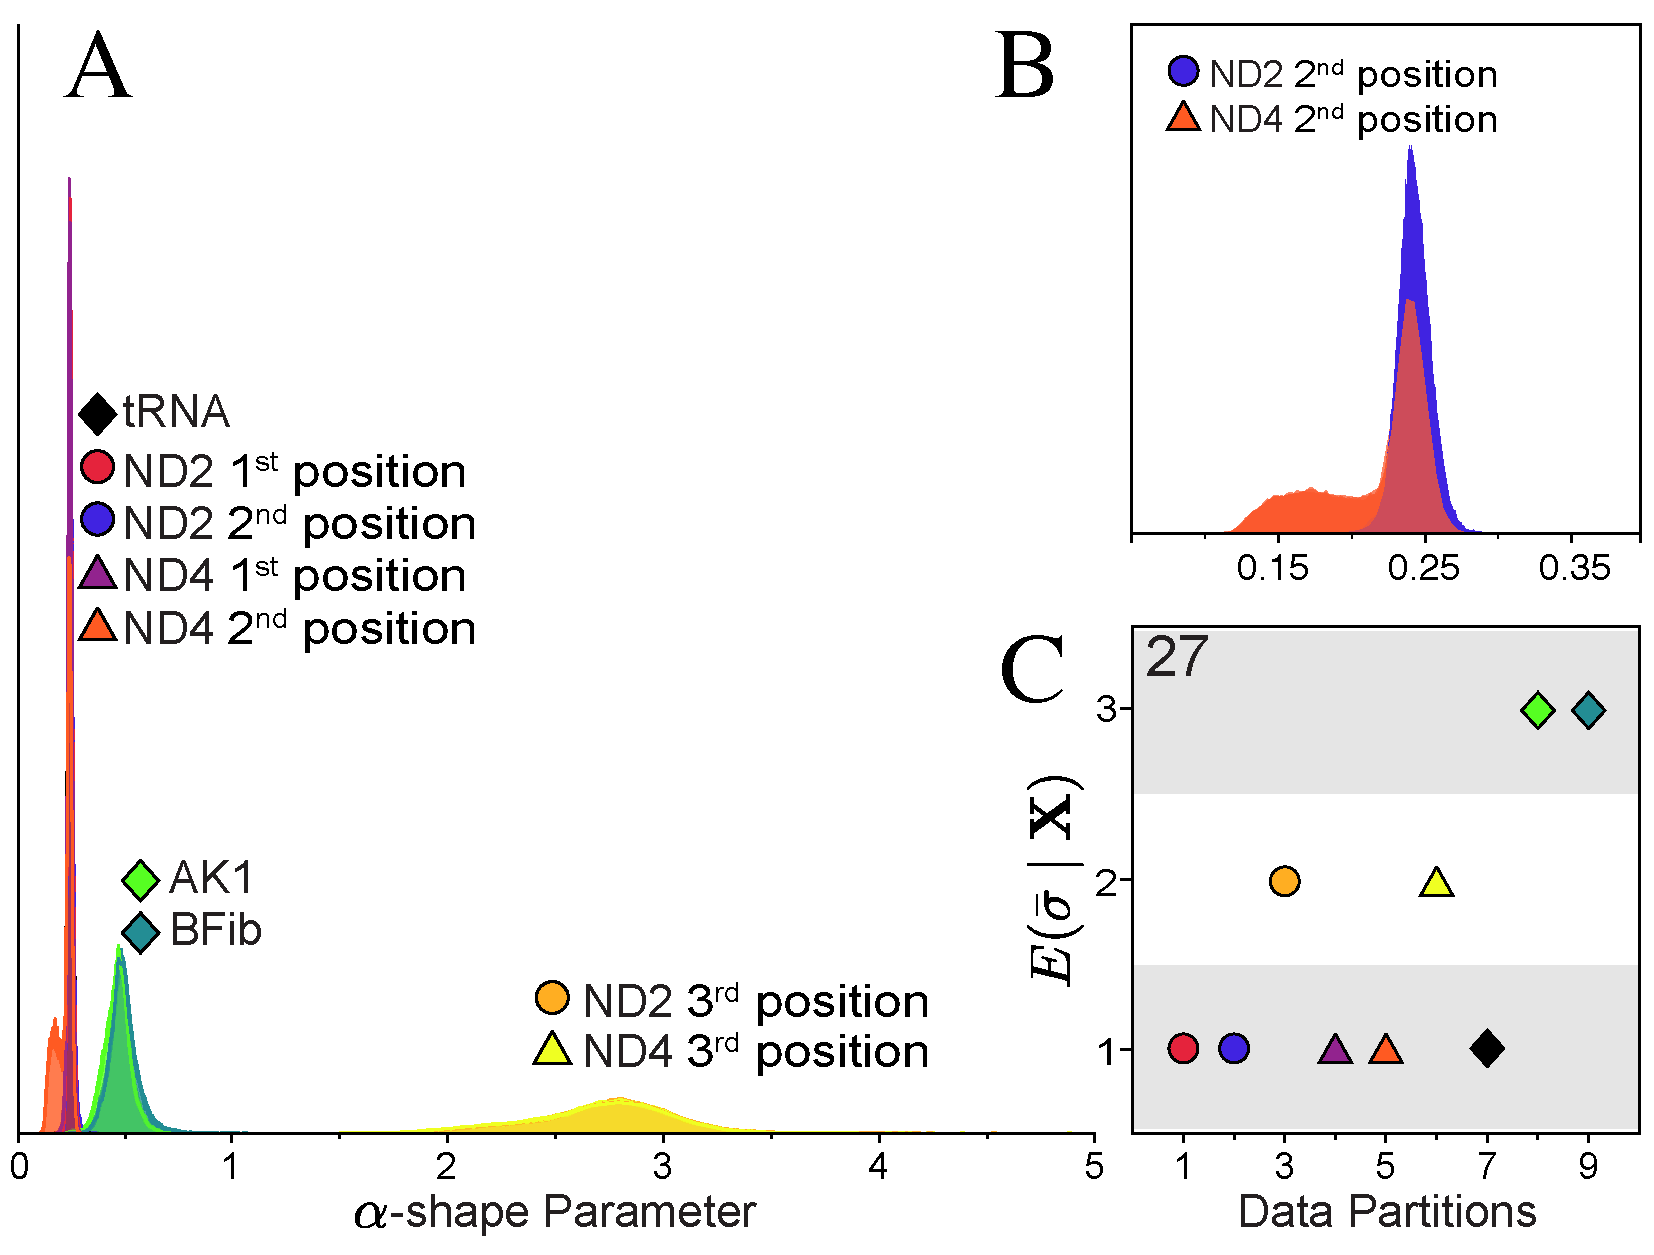
\includegraphics[width=120mm]{figures/figure_1} 
\end{figure} 

\newpage

\begin {center} 
{\sc Figure 2}
\end{center}

\vspace{1.0in}

\begin{figure}[h] 
\centering 
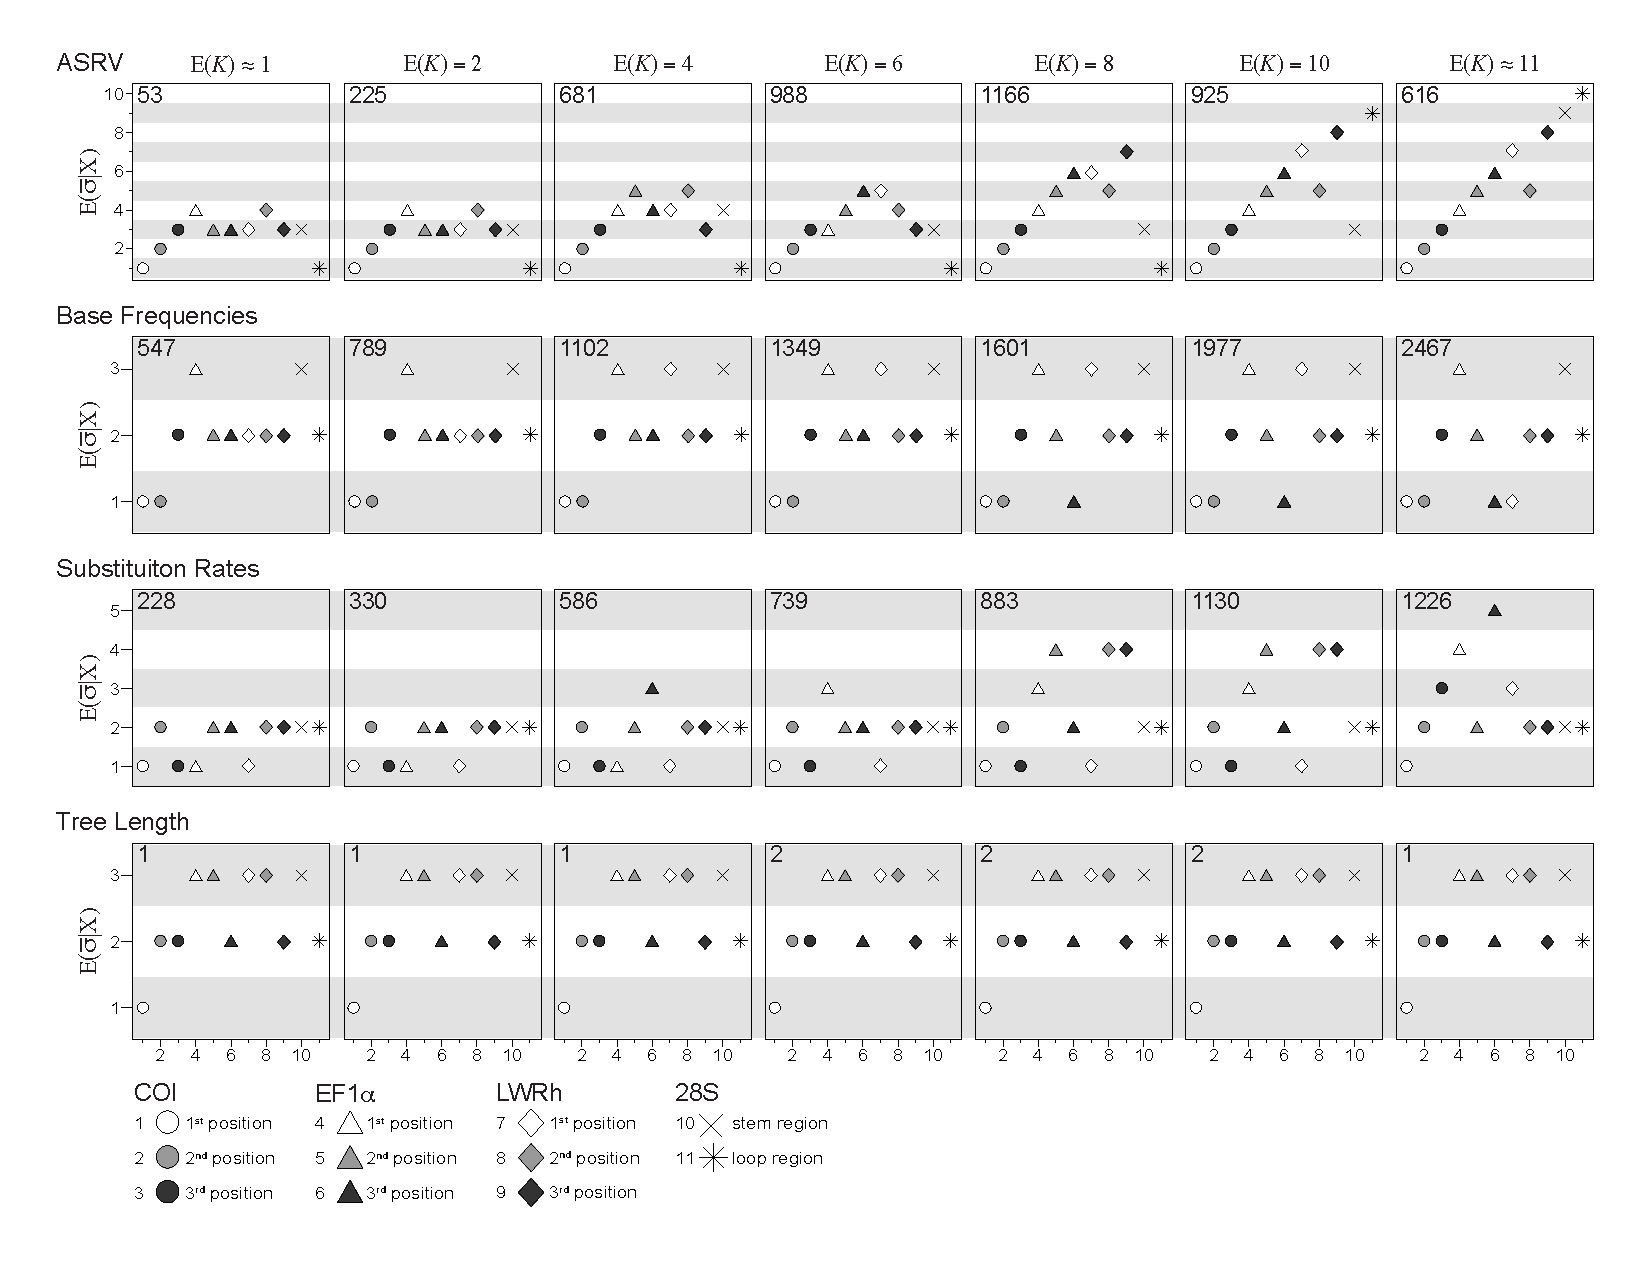
\includegraphics[angle=90, height=175mm]{figures/figure_2} 
\end{figure} 

\newpage

\begin {center} 
{\sc Figure 3}
\end{center}

\vspace{1.0in}

\begin{figure}[h] 
\centering 
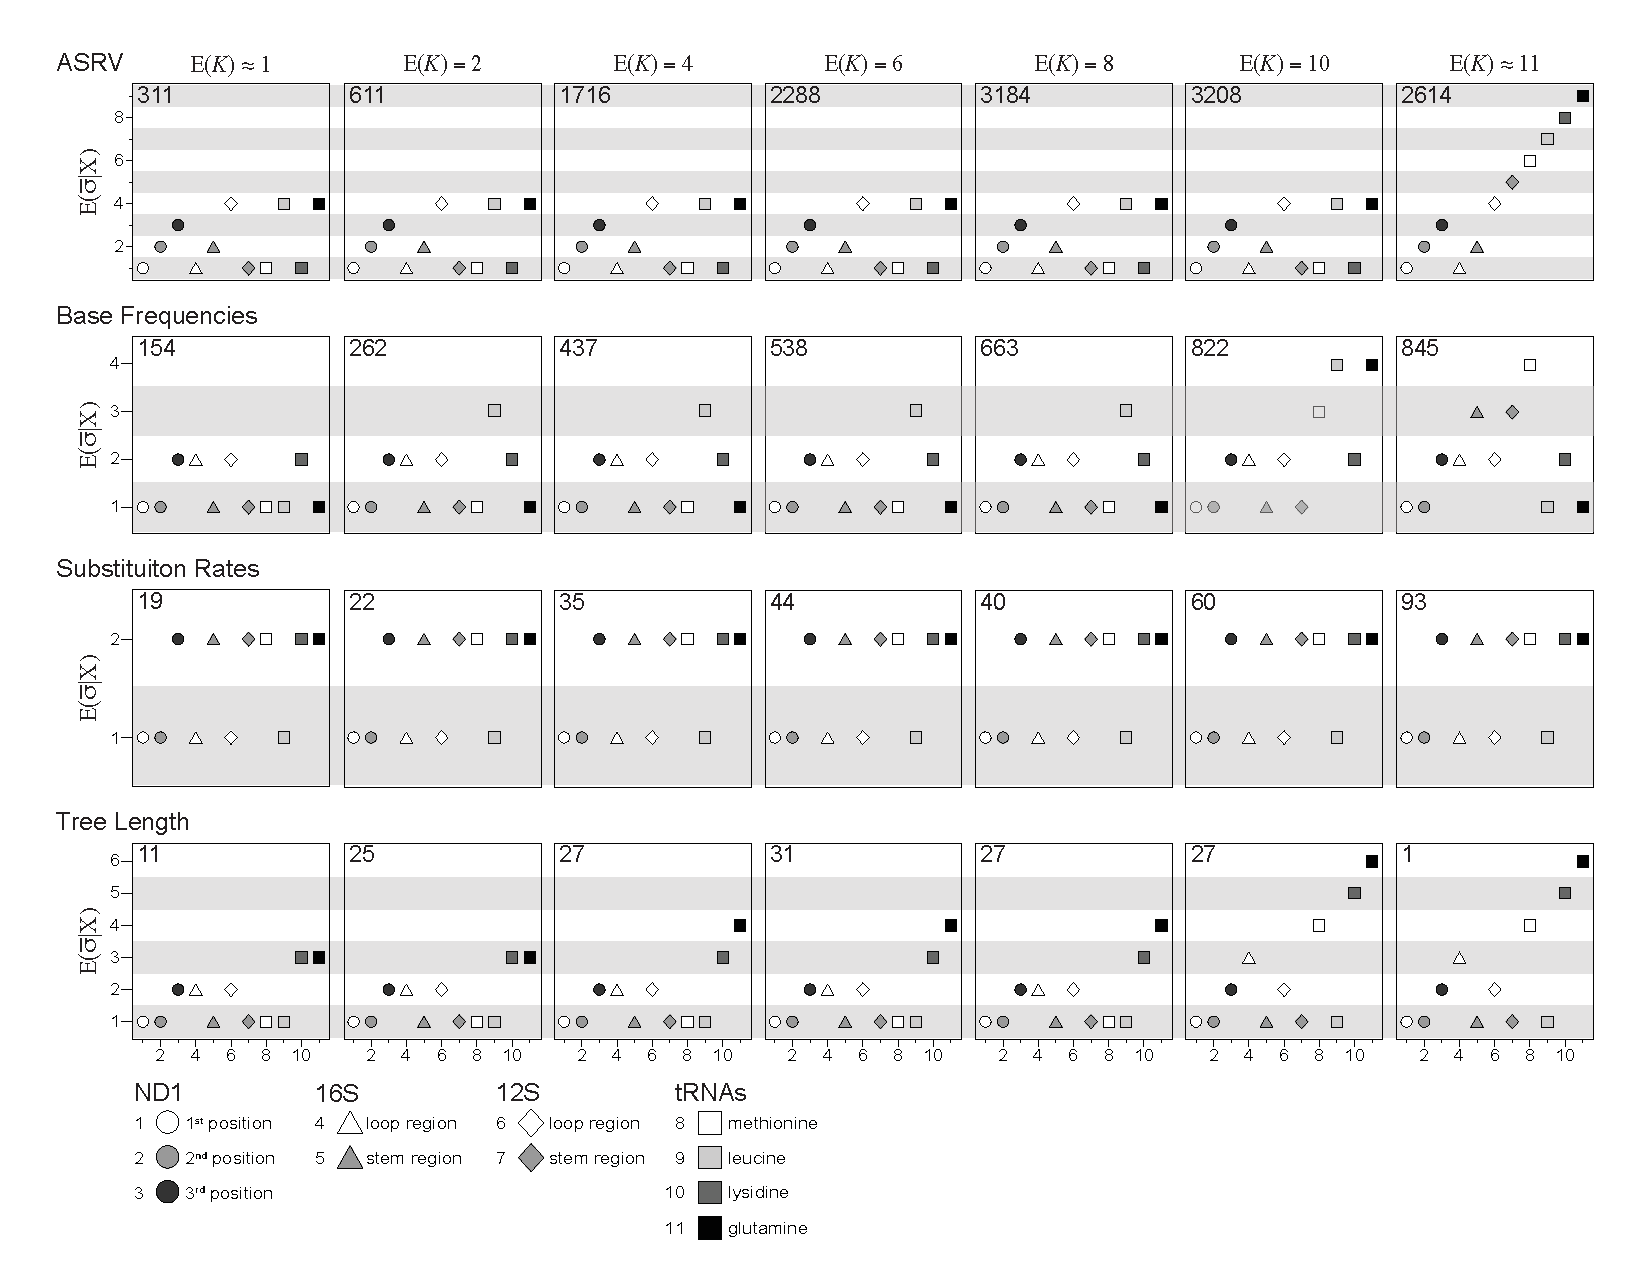
\includegraphics[angle=90, height=175mm]{figures/figure_3} 
\end{figure} 

\newpage

\begin {center} 
{\sc Figure 4}
\end{center}

\vspace{1.0in}

\begin{figure}[h] 
\centering 
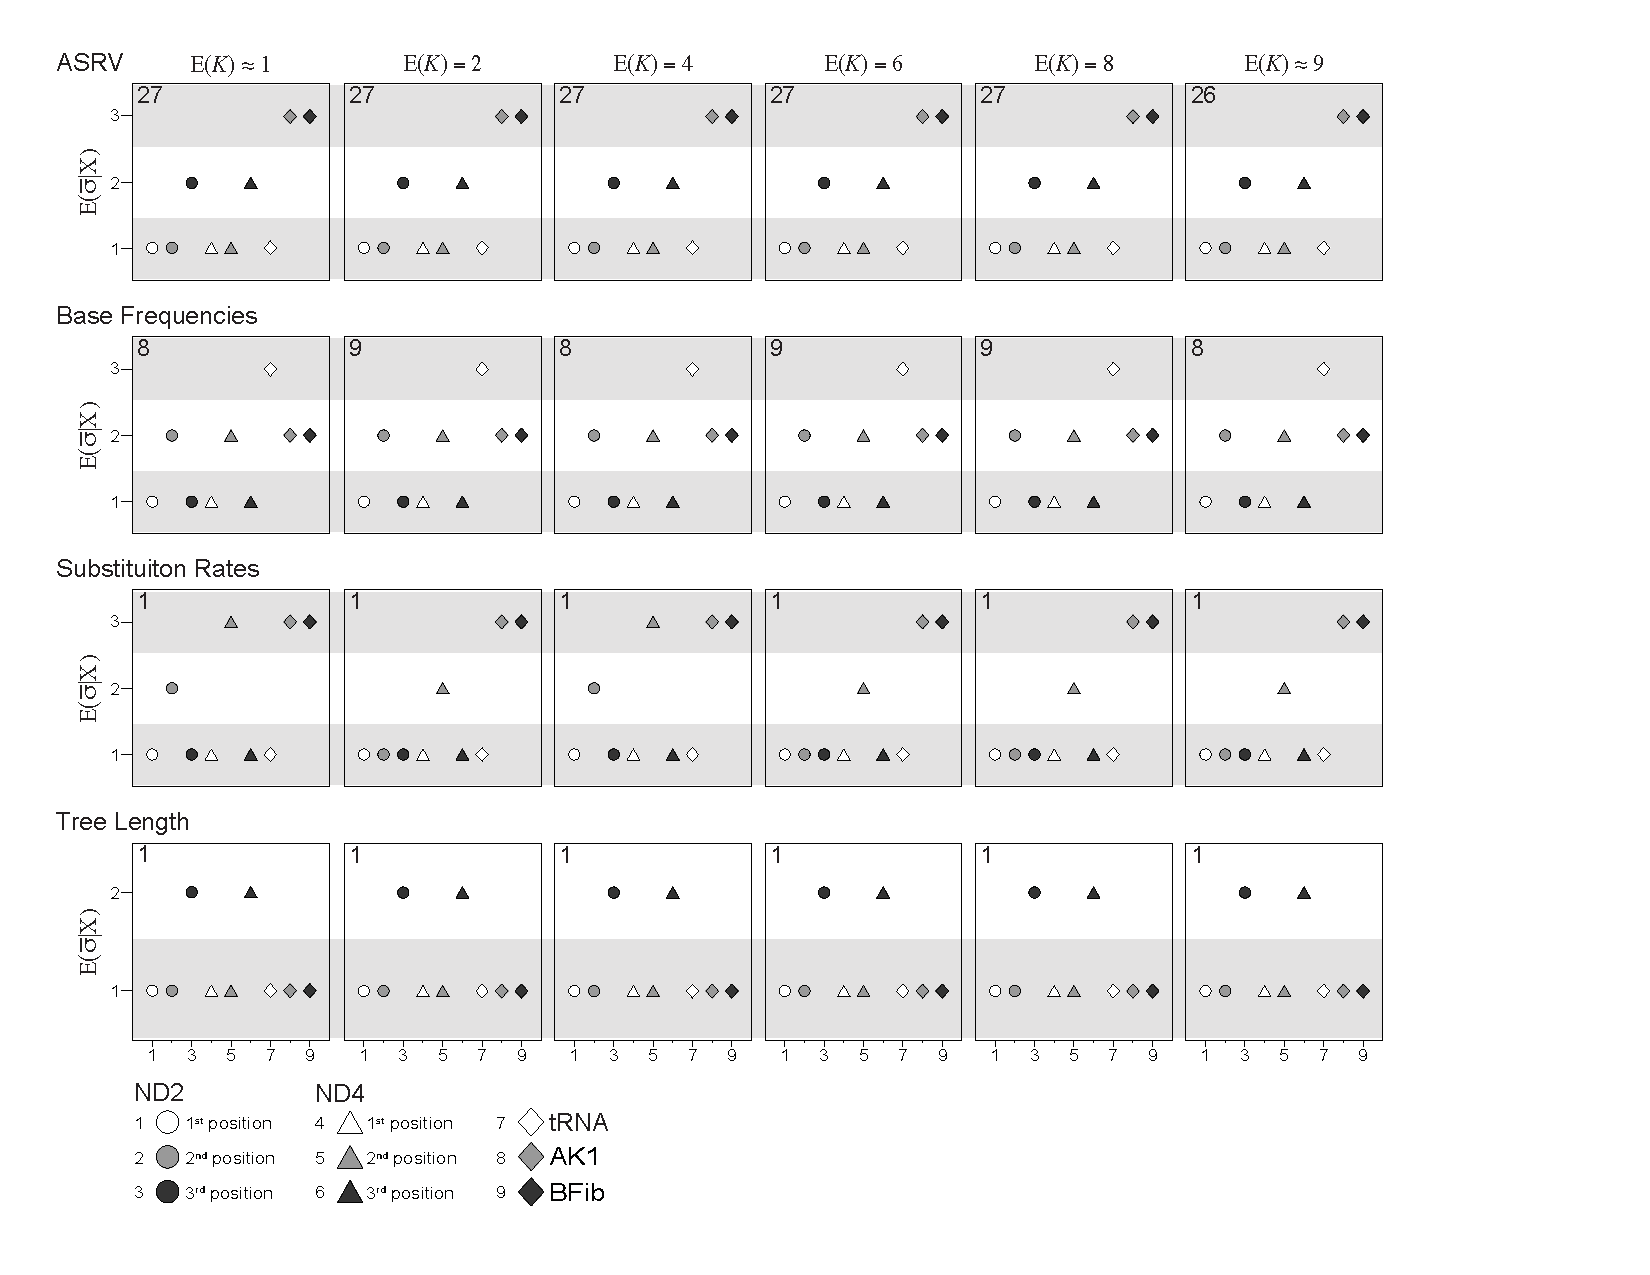
\includegraphics[angle=90, height=175mm]{figures/figure_4} 
\end{figure} 

\newpage

\begin {center} 
{\sc Figure 5}
\end{center}

\vspace{1.0in}

\begin{figure}[h] 
\centering 
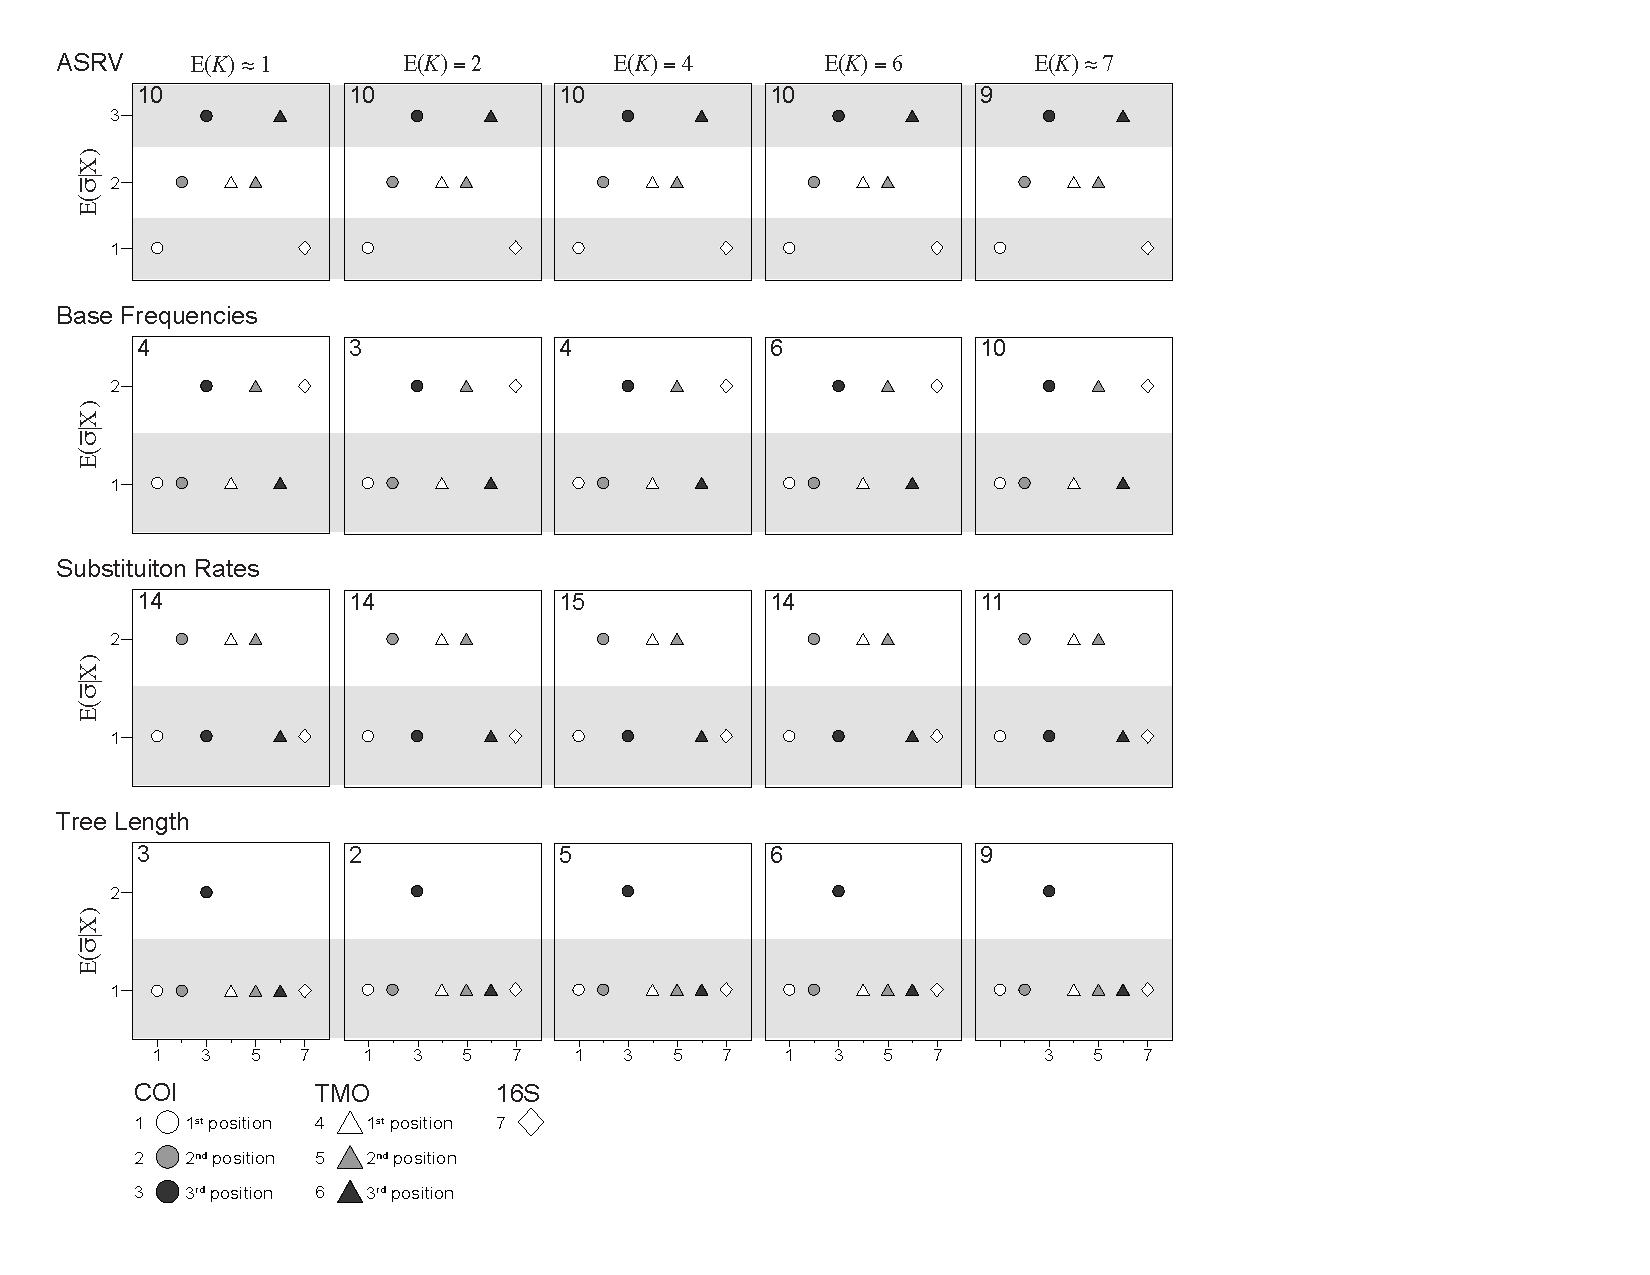
\includegraphics[height=175mm]{figures/figure_5} 
\end{figure} 

\newpage

\begin {center} 
{\sc Figure 6}
\end{center}

\vspace{1.0in}

\begin{figure}[h] 
\centering 
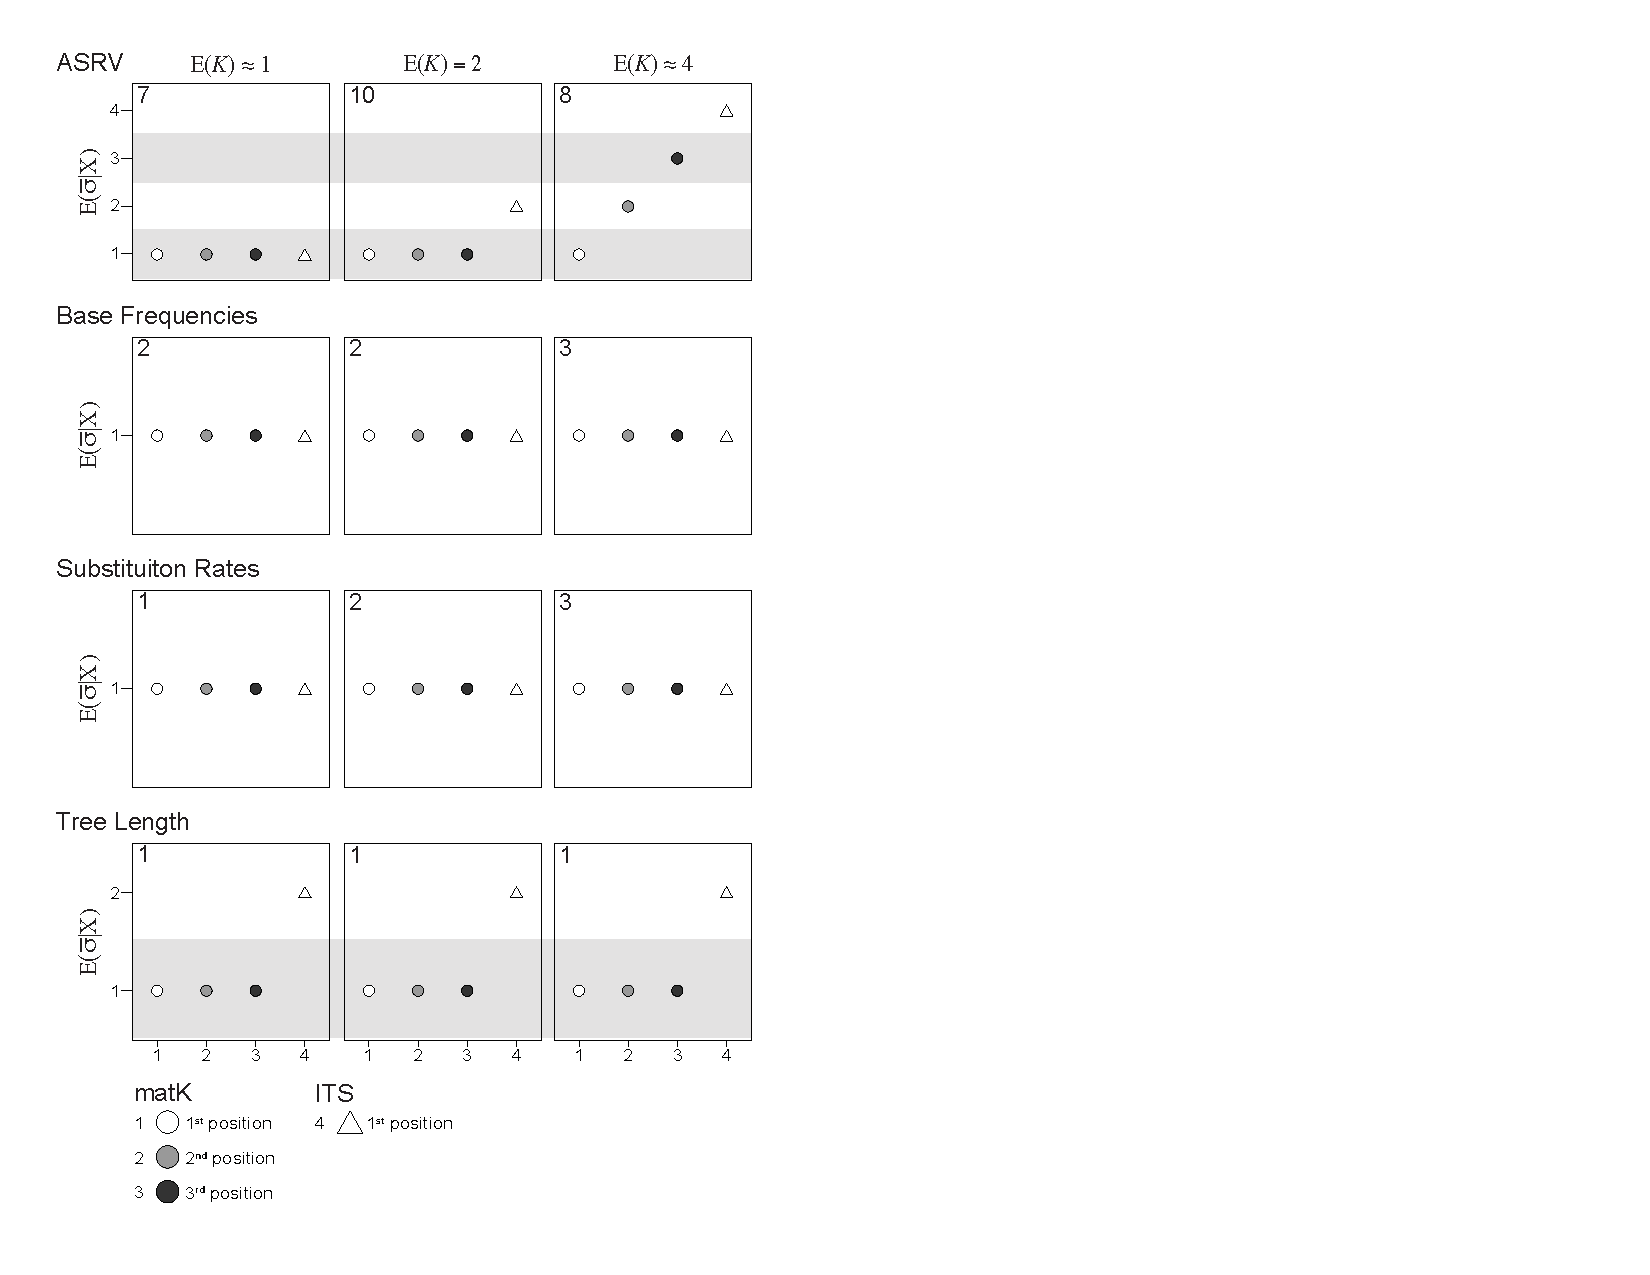
\includegraphics[height=175mm]{figures/figure_6} 
\end{figure} 




\end{document}


 

